%%%%%%%%%%%%%%%%%%%%%%%%%%%%%%%%%%%%%%%%%
%%%%%%%%%% Content starts here %%%%%%%%%%
%%%%%%%%%%%%%%%%%%%%%%%%%%%%%%%%%%%%%%%%%

\begin{frame}{Contents}
	\begin{itemize}
	  \item Introduction
	  \item Methodology
	  \item Results
	  \item Conclusion
	\end{itemize}
\end{frame}

\section{Introduction}

\begin{frame}{Social Addons?}
	\begin{itemize}
	  \item Like
	  \item Tweet
	  \item +1
	  \item Simple hyperlinks with icons that allow users to
share, recommend, rank or just comment any article they read
on a web page
	\end{itemize}
	    \begin{figure}
    \centering
        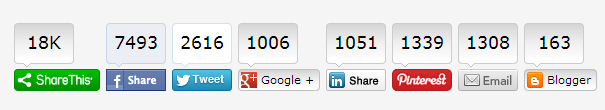
\includegraphics[width=.8\textwidth]{images/viral/social_plugins}
        \caption{Social addons}
        \label{fig:social_plugins}
    \end{figure}
\end{frame}

\begin{frame}{Conversion rate}
    \begin{itemize}
      \item Best known quality measure which shows what proportion of the
      visitors from different sources within a defined time period convert to
      specific marketing outcomes
      \item Conversion rates can be expressed in two different ways
      \begin{itemize}
        \item at visit level (visit or session conversion rate)
        \item the unique level (visitor conversion rate)
      \end{itemize}
      \item Sharing from users, the visits and conversions can be used
defining three coefficients usable in grading specific social
networks and the effect of social network on business
    \end{itemize}

\end{frame}

\begin{frame}{Effect of social networks}
\begin{scriptsize}
    \begin{equation}
    \label{conv_action}
    \frac{Conversions}{Social\ Actions}
    \end{equation}
    \ref{conv_action} How often social sharing leads to conversion.
    \begin{equation}
\label{conv_visits}
\frac{Conversions}{Social\ Visits}
\end{equation}

\ref{conv_visits} How often shared links on social networks leads to conversion.
 
\begin{equation}
\label{vists_actions}
\frac{Social\ Visits}{Social\ Actions}
\end{equation}

\ref{vists_actions} How often sharing on social networks leads to increased site traffic.
\end{scriptsize}
\end{frame}

\section{Methodology}

\begin{frame}{Methodology}{Hypothesis}
    Social addons increase the viral effect on some story (news)
    \begin{itemize}
      \item Hypothesis 1 - The time spent browsing social network sites
      increases, as the age decreases.
      \item Hypothesis 2 - Social sites are mostly visited from home, with the
      purpose of keeping a friendship.      
    \end{itemize}
\end{frame}

\begin{frame}{Methodology}{Hypothesis}
    \begin{itemize}
      \item Hypothesis 3 - More time spent browsing social network, leads to more
often usage of social addons.
      \item Hypothesis 4 - Among users of social sites, stories about life and
      entertainment are more popular than news and sports.
      \item Hypothesis 5 - By using social addons news are spreading faster (are
becoming viral).
    \end{itemize}
\end{frame}

\begin{frame}{Methodology}{Users}
    \begin{itemize}
      \item The research is conducted by surveying two independent
groups
    \begin{itemize}
        \item 565 Internet users (mainly consuming and sharing) 
        \item 24 Web site or blog owners (mainly offering or aggregating)
    \end{itemize}
        \item The research was conducted in September 2013 and lasted
3 weeks
    \end{itemize}
\end{frame}

\section{Results}

\begin{frame}{Results}{Results from Internet users}
      50.4\% male and 49.6\% female
      \begin{figure}
    \centering
        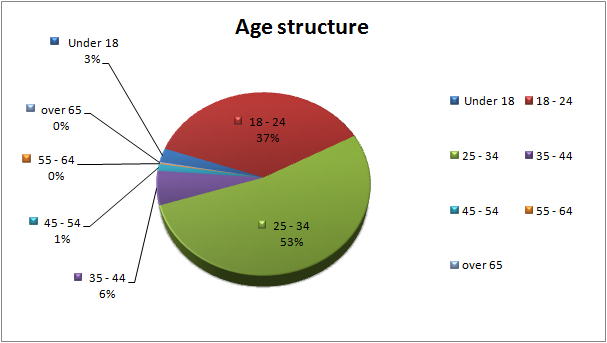
\includegraphics[width=.7\textwidth]{images/viral/age_structure}
        \caption{Age structure}
        \label{fig:age_structure}
    \end{figure}
\end{frame}

\begin{frame}{Results}{Results from Internet users}
      \begin{figure}
    \centering
        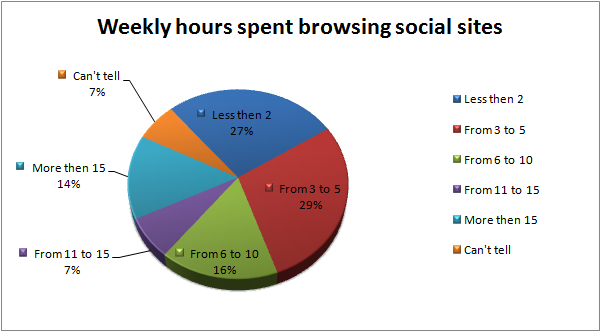
\includegraphics[width=.7\textwidth]{images/viral/weekly_hours}
        \caption{Weekly hours spent browsing social sites.}
        \label{fig:weekly_hours}
    \end{figure}
    Avarage 6.2 hours
\end{frame}

\begin{frame}{Results}{Results from Internet users}
      \begin{figure}
    \centering
        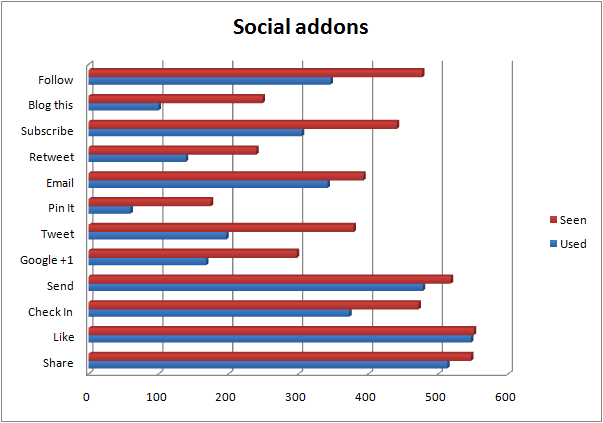
\includegraphics[width=.7\textwidth]{images/viral/social_addons}
        \caption{Social addons.}
        \label{fig:social_addons}
    \end{figure}
\end{frame}

\begin{frame}{Results}{Results from Internet users}
      \begin{figure}
    \centering
        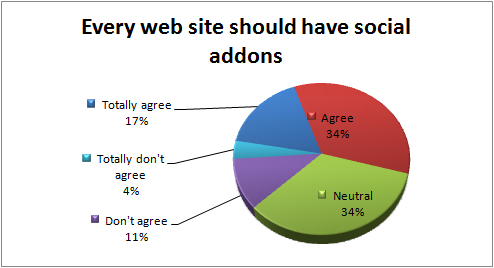
\includegraphics[width=.8\textwidth]{images/viral/every_web_site}
        \caption{Every web site should have social addons.}
        \label{fig:social_addons}
    \end{figure}
\end{frame}

\begin{frame}{Results}{Results from Internet users}
      \begin{figure}
    \centering
        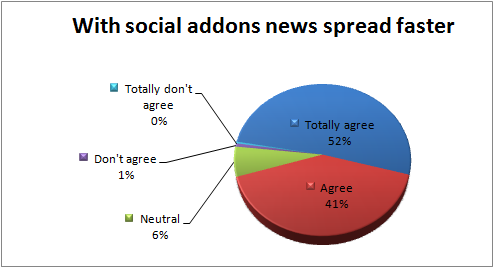
\includegraphics[width=.8\textwidth]{images/viral/news_spread_faster}
        \caption{With social addons news spread faster.}
        \label{fig:news_spread_faster}
    \end{figure}
\end{frame}

\begin{frame}{Results}{Results from web site owners}
Second questionnaire has total 24 responders (owners of web sites or blogs in
R. Macedonia)
      \begin{figure}
    \centering
        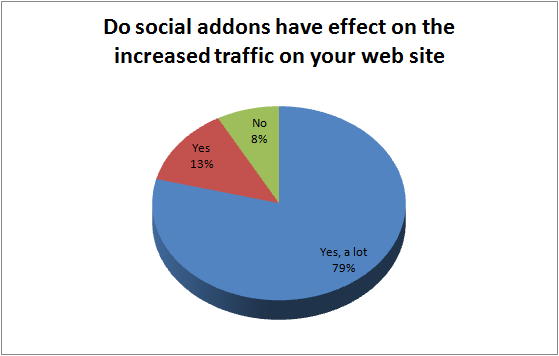
\includegraphics[width=.6\textwidth]{images/viral/effect}
        \caption{Do social addons have effect on the increased traffic on your web
site.}
        \label{fig:effect}
    \end{figure}
\end{frame}

\section{Conclusion}

\begin{frame}{Conclusion}
    Results from the survey are \textbf{confirming} most of the presented hypothesis
    \begin{itemize}
      \item The results for the age structure \textbf{doesn’t conclude} the first
      hypothesis
      \item The second hypothesis about \textbf{the location} of the users browsing
      social sites is \textbf{confirmed}, and the results are also showing that
      \textbf{friendship} is not the dominant motivation for browsing social
      sites, the \textbf{fun} is stated as most answered choice.
    \end{itemize}
\end{frame}

\begin{frame}{Conclusion}
    \begin{itemize}
      \item Users spending \textbf{most hours weekly} using social networks,
are \textbf{most often users} of social addons, confirming the third hypothesis.
        \item The fourth hypothesis concerned with the type of content shared is
        also confirmed, since \textbf{life style} and \textbf{fun} stories are most shared stories.
        \item The fifth and final hypothesis is confirmed both from users and
        from owners.
    \end{itemize}
\end{frame}

\begin{frame}{Questions}{}
    \begin{center}
    \vfill
    \huge{Thank you for your attention}
    \vfill    
    \Huge{Questions?}
    \end{center}
\end{frame}







